\documentclass[nobib]{tufte-handout}

\title{Föreläsning 2: Binomialsatsen, kompositioner, multinomialsatsen, och lådprincipen $\cdot$ 1MA020}

\author[Vilhelm Agdur]{Vilhelm Agdur\thanks{\href{mailto:vilhelm.agdur@math.uu.se}{\nolinkurl{vilhelm.agdur@math.uu.se}}}}

\date{17 januari 2023}


%\geometry{showframe} % display margins for debugging page layout

\usepackage{graphicx} % allow embedded images
  \setkeys{Gin}{width=\linewidth,totalheight=\textheight,keepaspectratio}
  \graphicspath{{graphics/}} % set of paths to search for images
\usepackage{amsmath}  % extended mathematics
\usepackage{booktabs} % book-quality tables
\usepackage{units}    % non-stacked fractions and better unit spacing
\usepackage{multicol} % multiple column layout facilities
\usepackage{lipsum}   % filler text
\usepackage{fancyvrb} % extended verbatim environments
  \fvset{fontsize=\normalsize}% default font size for fancy-verbatim environments

\usepackage{color,soul} % Highlights for text


\include{mathcommands.extratex}

\begin{document}

\maketitle% this prints the handout title, author, and date

\begin{abstract}
\noindent
Vi bevisar binomialsatsen med ett kombinatoriskt bevis. Vi fortsätter med att diskutera omordningar och kompositioner, från vilket vi härleder \emph{multi}nomialsatsen. Sedan introducerar vi lådprincipen, och använder den för att bevisa ett resultat om Ramseytalen och Erd\H{o}s-Szekeres sats.
\end{abstract}

\section{Binomialsatsen}

\begin{theorem}[Binomialsatsen]
  För varje heltal $n\geq 0$ gäller det att\sidenote[][]{Lägg märke till att vi inte är så precisa kring vad $x$ och $y$ är. I versionen ni lärde er i gymnasiet är de två reella tal, men egentligen är det här en likhet mellan polynom, som gäller mycket mer allmänt. Vi använder ju inte några specifika egenskaper hos de reella talen i det här beviset, bara räkneregler för polynom. När ni läser en kurs i algebra kommer ni se hur generellt den sortens räkningar fungerar.}
  $$(x + y)^n = \sum_{k=0}^n \binom{n}{k}x^{n-k}y^k$$
  \begin{proof}
    Studera uttrycket
    $$(x + y)^n = (x + y)(x + y)\ldots(x + y).$$

    Vad är det vi gör när vi expanderar ut detta uttrycket? Jo, vi väljer för varje parentes om vi tar ett $x$ eller ett $y$ -- eller uttryckt i kombinatoriska termer, vi bildar ett ord ur alfabetet $\{x, y\}$. Så för $n = 3$ får vi till exempel att
    $$(x+y)(x+y)(x+y) = xxx + xxy + xyy + yxx + yxy + yyy.$$

    Sedan kommer vi ihåg att multiplikation är kommutativt, så $xyy = yxy$. Alltså spelar det ingen roll i vilken ordning vi gjorde valen, bara hur många gånger vi valde $x$ och hur många gånger vi valde $y$.\sidenote[][]{Alltså, formulerat på ett annat sätt, etiketterna av ``när valdes vilken'' spelar ingen roll.}

    Så antalet gånger vi får en term som är lika med $x^{n-k}y^k$ kommer alltså vara antalet $\{x, y\}$-strängar med $k$ stycken $y$. Det antalet är så klart samma som antalet sätt att välja $k$ platser att skriva $y$ ur den totala mängden av $n$ platser -- det vill säga $\binom{n}{k}$.

    Vi har alltså sett att koefficienten framför $x^{n-k}y^k$ när vi förenklat uttrycket kommer att vara $\binom{n}{k}$. Eftersom detta argument fungerar för varje $k$ har vi bevisat satsen.
  \end{proof}
\end{theorem}

\begin{example}
  Ge ett algebraiskt och ett kombinatoriskt bevis för att
  $$3^n = \sum_{k=0}^n \binom{n}{k}2^k.$$

  \begin{proof}[Kombinatoriskt bevis]
    Låt oss räkna antalet ternära strängar\sidenote[][]{Det vill säga strängar med alfabetet $\{0,1,2\}$.} av längd $n$ på två olika sätt. Det enkla sättet är att använda multiplikationsprincipen -- för varje bokstav har vi tre val, och vi behöver välja $n$ gånger, alltså blir produkten av antalet val för varje gång $3^n$.

    Ett annat sätt att räkna detta är att dela upp efter hur många ettor ordet innehåller. Först väljer vi antalet ettor, sedan väljer vi var ettorna skall stå, och till sist väljer vi vad resten av bokstäverna skall vara för något.

    Givet att vi vet att vi skall ha $k$ stycken ettor, och vi vet var de skall stå, så har vi $n-k$ bokstäver kvar att göra ett val för -- och nu har vi bara två val, eftersom vi inte får välja ettor utan bara nollor och tvåor. Så enligt multiplikationsprincipen multiplicerar vi antalet val vi har i varje fall och får att det finns $2^{n-k}$ sätt att fylla i resten av ordet med nollor och tvåor.

    Givet att vi vet att vi skall ha $k$ stycken ettor, hur många olika strängar kan vi skapa? Antalet sätt att välja var ettorna skall stå är precis antalet kombinationer av $k$ element från mängden av platser, $[n]$, och vi vet att det är $\binom{n}{k}$. När vi väl valt var ettorna skall stå kan vi fylla i resten på $2^{n-k}$ sätt, som vi såg i föregående stycket, så multiplikationsprincipen ger oss att det måste finnas $\binom{n}{k}2^{n-k}$ strängar av längd $n$ med $k$ stycken ettor.

    Till slut vet vi att det totala antalet ternära strängar måste vara summan av detta över alla $k$, enligt additionsprincipen. Så om vi summerar detta får vi att det finns
    $$\sum_{k=0}^n \binom{n}{k}2^{n-k}$$
    ternära strängar. Efter att ha tillämpat likheten $\binom{n}{k} = \binom{n}{n-k}$ och vänt på indexeringen i summan ser vi att detta är precis höger led i ekvationen vi gav.
  \end{proof}

  \begin{proof}[Algebraiskt bevis]
    Vi använder binomialsatsen och ser att
    \begin{align*}
      3^n &= (1+2)^n\\
      &= \sum_{k=0}^n \binom{n}{k}1^{n-k}2^k = \sum_{k=0}^n \binom{n}{k}2^k.
    \end{align*}
  \end{proof}
\end{example}

\section{Omordningar}

\begin{definition}
  En omordning\sidenote[][]{Engelska \emph{rearrangement}, det verkar inte finnas ett helt inarbetat svenskt ord för detta, så omordning får fungera, om än klumpigt.} av en $X$-sträng $s$ är en annan $X$-sträng $s'$ där varje element i $X$ förekommer lika många gånger i $s'$ som i $s$. Specifikt måste alltså $s$ och $s'$ vara av samma längd.
\end{definition}

\begin{example}
  Det finns sex omordningar av $ABBA$:
  $$ABBA, ABAB, AABB, BAAB, BABA, BBAA.$$
\end{example}

\begin{proposition}\label{proposition_count_binary_rearrangements}
  Om $s$ är en binär sträng av längd $n$ med $k$ stycken ettor finns det $\binom{n}{k}$ stycken omordningar av $s$.
  \begin{proof}
    Vi behöver helt enkelt räkna antalet binära strängar av längd $n$ som har $k$ stycken ettor. För att konstruera en sådan behöver vi helt enkelt välja på vilka platser det skall stå en etta -- alltså välja en delmängd av $k$ platser av de totalt $n$ platserna. Detta vet vi att vi kan göra på $\binom{n}{k}$ sätt.
  \end{proof}
\end{proposition}

\section{Kompositioner}

Antag att vi vill fördela ut $n$ stycken osärskiljbara objekt bland $k$ särskiljbara människor.

\begin{example}
  Tre stycken lärare konkurrerar om två stycken äpplen de har fått av sina elever. På hur många olika sätt kan äpplena fördelas ut?

  Här är $n=2$ och $k=3$. Det finns sex olika sätt:
  \begin{table}[h]
    \begin{tabularx}{0.7\textwidth}{ccc}
    Äpplen för A & Äpplen för B      & Äpplen för C \\ 
    \midrule
    2 & 0 & 0\\
    1 & 1 & 0\\
    1 & 0 & 1\\
    0 & 2 & 0\\
    0 & 1 & 1\\
    0 & 0 & 2
    \end{tabularx}
    \end{table}
\end{example}

\begin{definition}
  En \emph{multi-mängd} är en mängd där ett objekt kan vara med mer än en gång.\sidenote[][]{Alltså är $\{1,1,2\}$ en annan multimängd än $\{1,2\}$, trots att de är samma som mängder.} En \emph{multi-delmängd} till en (multi-)mängd är en delmängd som kan innehålla samma objekt ur mängden flera gånger.\sidenote[][]{Så till exempel är $\{a,b,a,c\}$ en multidelmängd till $\{a,b,c,d\}$.}

  Vi kan betrakta ett sätt att fördela $n$ stycken osärskiljbara föremål mellan $k$ särskiljbara personer som ett sätt att välja en multi-delmängd av storlek $n$ ur mängden av personer. Vi kan också ekvivalent betrakta det som ett sätt att skriva $n$ som summan av $k$ stycken ickenegativa heltal där ordningen i summan spelar roll.\sidenote[][]{Alltså att $1 + 0 + 3$ och $0 + 1 + 3$ är olika sätt att skriva $4$.}
\end{definition}

\begin{proposition}\label{proposition_indist_objs_dist_persons}
  Det finns $\binom{n+k-1}{k-1} = \binom{n+k-1}{n}$ multi-delmängder av storlek $n$ till en mängd med $k$ element.Detta räknar alltså också sätt att fördela $n$ osärskiljbara föremål mellan $k$ särskiljbara personer.

  \begin{proof}
    Metoden för det här beviset brukar kallas för ett pinnar-och-stjärnor-argument.\sidenote[][]{Engelska \emph{stars and bars argument}.}

    Vi studerar ord ur alfabetet $\{*,|\}$ med $k-1$ stycken pinnar och $n$ stycken stjärnor. Till exempel om $n=6$ och $k=5$
    $$**||*|*|**.$$

    Vi tolkar detta ordet som en fördelning av föremål till personer såsom följer: Person ett får alla  stjärnor innan första strecket, person två alla mellan första och andra strecket, och så vidare, tills person $k$ får alla stjärnor efter det sista strecket. I vårt exempel får alltså person ett två föremål, person två inga, person tre och fyra ett var, och person fem får två.

    Detta etablerar en bijektion mellan våra ord och fördelningarna till personer. Vi vet från Proposition \ref{proposition_count_binary_rearrangements}\sidenote[][]{Den propositionen handlar om binära strängar, men vi har alfabetet $\{*,|\}$ -- det spelar så klart ingen roll för antalet vad vi kallar våra bokstäver.} hur man räknar antalet sådana ord -- våra ord har längd $n + k -1$ (de innehåller $n$ stjärnor och $k-1$ streck) och $k-1$ av dem är av ena typen, så det måste finnas totalt $\binom{n + k - 1}{k - 1}$ ord, och alltså lika många fördelningar.
  \end{proof}
\end{proposition}

\begin{example}
  Hur många lösningar har ekvationen $x + y + z = 15$, ifall vi kräver att $x$, $y$, och $z$ alla skall vara positiva heltal?

  Vi kan se det här som en variant av problemet med att fördela osärskiljbara objekt mellan särskiljbara personer, där objekten är ettor och personerna är våra tre variabler. 
  
  Vi börjar med att ge varje variabel en etta, eftersom alla måste vara större än noll. Sedan har vi tolv ettor kvar att fördela mellan tre variabler, så Proposition \ref{proposition_indist_objs_dist_persons} säger oss att det finns $\binom{12 + 3 -1}{3 - 1} = \binom{14}{2} = 91$ lösningar.
\end{example}

\begin{definition}
  I allmänhet är antalet sätt att skriva $n$ som en summa av ett godtyckligt antal positiva heltal, där ordningen vi skrivar summan i spelar roll\sidenote[][]{$1+4$ och $4+1$ är alltså olika kompositioner av $5$.}, antalet \emph{kompositioner}\sidenote[][]{Inte att blanda ihop med \emph{kombinationer}, trots ordens snarlikhet.} av $n$. Vi studerade alltså just antalet kompositioner av längd $3$ av $15$.
\end{definition}

\section{Multinomialkoefficienter}

\begin{example}
  Hur många omordningar finns det av ordet $SPAPASTA$?\sidenote[][]{Ursprungligen ville jag ha det rimligare ordet \emph{pastasås}, men \LaTeX\ gillar visst inte \emph{Å} i ekvationer.}

  Det har $2$ stycken $S$ och $P$, $3$ stycken $A$, och ett $T$. Vi kan skapa en omordning av detta ordet genom att först välja var vi placerar $A$na -- det kan vi göra på $\binom{8}{3}$ sätt, eftersom vi har åtta platser och tre $A$n. När vi placerat ut dem har vi $8 - 3 = 5$ sätt att placera ut våra två $S$, så vi har $\binom{5}{2}$ val för hur vi gör det.

  Likaledes har vi $\binom{3}{2}$ sätt att placera ut våra $P$n, och till slut $\binom{1}{1}$ enda sätt att placera ut vårt $T$. Sammantaget blir det alltså
  \begin{align*}
    \binom{8}{3}\binom{5}{2}\binom{3}{2}\binom{1}{1} &= \frac{8!}{3!5!}\frac{5!}{2!3!}\frac{3!}{2!1!}\frac{1!}{1!0!}\\
    &= \frac{8!}{3!2!2!1!}
  \end{align*}
\end{example}

\begin{definition}
  För varje heltal $n$ och varje samling av heltal $k_1, k_2, \ldots, k_r$ sådana att $k_1 + k_2 + \ldots + k_r = n$ betecknar vi \emph{multinomialkoefficienten} med
  $$\binom{n}{k_1, k_2, \ldots, k_r} = \frac{n!}{k_1!k_2!\ldots k_r!}.$$

  Notera att våra vanliga binomialkoefficienter är specialfallet när $r=2$,
  $$\binom{n}{k} = \binom{n}{k, n-k} = \binom{n}{n-k}.$$
\end{definition}

\begin{proposition}
  Antag att $s$ är en $X$-sträng av längd $n$, som innehåller $k_1$ stycken $x_1$, $k_2$ stycken $x_2$, och så vidare, upp till $k_r$ stycken $x_r$ -- så $k_1 + k_2 + \ldots k_r = n$. Antalet omordningar av $s$ ges av multinomialkoefficienten $\binom{n}{k_1, k_2, \ldots, k_r}$.

  \begin{proof}
    Låt $R$ vara antalet omordningar av $s$. Vi använder återigen ``räkna samma sak på två olika sätt''-metoden. Den här gången är vad vi vill räkna antalet permutationer av längd $n$ ur alfabetet\sidenote[][]{Så i fallet där vårt ord är $SPAPASTA$ blir $$X' = \{S^1, S^2, P^1, P^2, A^1, A^2, A^3, T^1\}.$$
    
    Vi tar helt enkelt varje bokstav och ger den en etikett, så att bokstäverna blir särskiljbara.}
    \begin{align*}
      X' = \{&x_1^1, x_1^2, \ldots, x_1^{k_1},\\
             &x_2^1, x_2^2, \ldots, x_2^{k_2},\\
             &\qquad\vdots\\
             &x_r^1, x_r^2, \ldots, x_r^{k_3}\}.
    \end{align*}

    Eftersom $X'$ har exakt $n$ bokstäver vet vi att antalet permutationer av det alfabetet är precis $n!$.

    Låt oss nu räkna på ett mer komplicerat sätt. Vi kan också skapa oss en permutation av $X'$ genom att först välja en omordning av $s$, och sedan välja ett sätt att sätta etiketter på bokstäverna i den omordningen.\sidenote[][]{Så vi väljer en omordning av $SPAPASTA$, till exempel $ASPTAPAS$, och sätter sedan etiketter på bokstäverna för att få till exempel $A^2S^1P^2T^1A^1P^1A^3S^2$, vilket är en permutation av $X'$.}

    Om vi bara studerar våra $x_1$ i omordningen av $s$ så har vi $k_1$ stycken, och vi skall sätta etiketter mellan $1$ och $k_1$ på dem. Det kan vi göra på $k_1!$ sätt. Det samma gäller för varje annan bokstav, så multiplikationsprincipen säger oss att det totala antalet sätt att sätta etiketter måste vara $k_1!k_2!\ldots k_r!$. Det totala antalet permutationer av $X'$ måste alltså vara $R$, antalet omordningar, gånger detta, så vi har sett att 
    $$n! = Rk_1!k_2!\ldots k_r!$$
    och om vi löser detta för $R$ får vi precis den sökta satsen.
  \end{proof}
\end{proposition}

\begin{theorem}[Multinomialsatsen]
  Det gäller att
  $$(x_1 + x_2 + \ldots + x_r)^n = \sum_{\substack{k_1, k_2, \ldots, k_r \geq 0\\k_1 + k_2 + \ldots + k_r = n}} \binom{n}{k_1, k_2, \ldots, k_r} x_1^{k_1} x_2^{k_2} \ldots x_r^{k_r}$$

  \begin{proof}
    Precis samma argument som för binomialsatsen fungerar här.
  \end{proof}
\end{theorem}

\section{Lådprincipen}

\begin{theorem}[Lådprincipen]\sidenote[][]{Också kallad Dirichlets lådprincip, efter den tyske matematikern Peter Gustav Lejeune Dirichlet. Eller på engelska ``the pigeonhole principle'' -- vilket onekligen är ett mer målande namn än vår svenska lådprincip.}
  Om vi har $m$ stycken objekt som skall fördelas i $n$ lådor, och $m > n$, så kommer någon låda behöva innehålla mer än ett objekt.
\end{theorem}

\begin{example}
  Om det finns tretton studenter i rummet måste åtminstone två av dem fylla år i samma månad. Här är studenterna objekten och årets månader lådorna.\sidenote[][]{Här önskar jag att kursen gick på engelska, så jag kunde skriva, såsom i förra föreläsarens anteckningar, att ``students are pigeons''.}
\end{example}

\begin{theorem}[Generaliserade lådprincipen]
  Om vi har $m$ objekt som skall fördelas i $n$ lådor, och $m > kn$, så måste åtminstone en av lådorna innehålla minst $k+1$ objekt.
\end{theorem}

\begin{example}
  Om det finns tjugofem studenter i rummet måste det finnas minst en månad i vilken tre eller fler av dem fyller år.
\end{example}

\begin{example}
  Antag att fem punkter placeras i en liksidig triangel med sidlängd ett. Då finns det två punkter vars avstånd mellan varandra är högst $\frac{1}{2}$.

  Dela upp triangeln i fyra bitar, enligt figuren.
  \begin{figure}
    \centering
    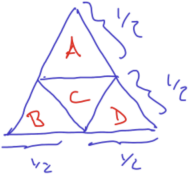
\includegraphics[width = 0.3\textwidth]{graphics/pigeonhole_principle_equilat_triangle.png}
    \caption{Figur tagen från förra föreläsarens föreläsningsanteckningar.}
  \end{figure}
  Lådprincipen säger oss att det måste finnas en av dessa bitar som innehåller minst två punkter. Men om de ligger i samma bit måste deras avstånd mellan varandra vara högst $\frac{1}{2}$.
\end{example}

\begin{example}
  För varje mängd av fem punkter på en sfär finns det ett halvklot som innehåller minst fyra av punkterna.

  Välj två av de fem punkterna godtyckligt och rita storcirkeln som passerar genom dem. Denna delar upp jorden i två halvklot, så lådprincipen säger oss att ett av dessa halvklot måste innehålla minst två av de återstående tre punkterna. Det halvklotet har alltså de två punkterna vi ritade storcirkeln genom och minst två punkter till, för totalt minst fyra.
\end{example}

\begin{example}\label{example_R33_is_6}
  I varje grupp av sex personer finns det antingen en grupp av tre personer som alla är vänner eller en grupp av tre personer som alla inte är vänner.\sidenote[][]{Vi antar här att ``är vänner''-relationen är symmetrisk, det vill säga att om jag är vän med dig är du vän med mig. Förhoppningsvis är det antagandet sant på universitetet, även om det inte var sant i mellanstadiet.}

  Välj en godtycklig person i gruppen. Enligt lådprincipen måste det antingen finnas tre personer som hon inte är vän med, eller tre personer som hon är vän med.

  Ifall det finns tre personer som hon inte är vän med har vi två fall -- antingen är alla tre vänner med varandra, i vilket fall vi är klara, eller så finns det ett par av dem som inte känner varandra. Men i så fall bildar det paret, tillsammans med vår första person, en grupp av tre personer som alla inte känner varandra.

  Ifall det finns tre personer som hon är vän med resonerar vi på samma vis. Antingen är ingen av de tre personerna vänner med varandra, i vilket fall vi hittat vår grupp, eller så finns det ett par som känner varandra, och i så fall bildar det paret tillsammans med vår första person en triangel som känner varandra.
\end{example}

Vad vi just studerat är det enklaste fallet av Ramseys sats.\sidenote[][-2cm]{Namngiven efter Frank P. Ramsey, som var en fascinerande person som hann bli vän med Wittgenstein och Keynes och finna viktiga resultat inom ekonomi, matematik, och filosofi innan sin bortgång vid 26 års ålder.} Låt oss definiera en lite mer allmän version av problemet.

\begin{definition}
  För varje par av positiva heltal $r$ och $s$ är $R(r,s)$ det minsta heltalet sådant att det för alla mängder $X$ av storlek minst $R(r,s)$ utrustade med en symmetrisk och reflexiv relation $\sim$ antingen existerar $A \in \binom{X}{r}$ sådant att $a \sim a'$ för alla $a, a' \in A$, eller existerar $B \in \binom{X}{s}$ sådant att $b \not\sim b'$ för alla $b\neq b'$ i $B$.\sidenote[][-2.2cm]{Så, för varje par av positiva heltal $r$ och $s$ är $R(r,s)$ det minsta antalet personer man behöver bjuda in på en fest för att det skall finnas antingen en grupp av $r$ personer som alla känner varandra, eller en grupp av $s$ personer där ingen känner någon annan i gruppen.
  
  Eller mer formellt, formulerat i termer av grafer:

  $R(r,s)$ är det minsta talet sådant att varje graf $G$ med minst $R(r,s)$ noder antingen innehåller en klick av storlek $r$ eller en oberoende mängd av storlek $s$.}
\end{definition}

Vad Exempel \ref{example_R33_is_6} visade är alltså att $R(3,3) = 6$. Vad Ramseys sats säger i allmänhet är att $R(r,s)$ är ändligt.\sidenote[][]{Problemet att beräkna exakt vad $R(r,s)$ är är extremt svårt -- vi vet att $R(4,4) = 18$, men kan inte bestämma $R(5,5)$ mer exakt än att det är mellan $43$ och $48$.}

\begin{theorem}[Ramseys sats]\label{ramseys_theorem}
  För varje $r, s \geq 1$ är $R(r,s) < \infty$.
\end{theorem}

\begin{theorem}[Erd\H{o}s-Szekeres]
  För alla $r,s \geq 1$ gäller det att varje följd av $(r-1)(s-1) + 1$ distinkta reella tal antingen innehåller en ökande delföljd av längd $r$ eller en minskande delföljd av längd $s$.\sidenote[][]{Med en ökande delföljd till följden $a_1, a_2, \ldots, a_N$ menar vi rent konkret en följd av index $1 \leq n_1 < n_2 < n_k \leq N$ sådan att $a_{n_1} < a_{n_2} < \ldots < a_{n_k}$, och motsvarande för en minskande delföljd.}

  \begin{proof}
    Kalla vår talföljd $n_1, n_2, \ldots, n_{(r-1)(s-1)+1}$. Ge varje $n_i$ en etikett $(a_i, b_i)$ som följer: $a_i$ är längden av den längsta ökande delföljden som slutar i $n_i$, och $b_i$ är längden av den längsta minskande delföljden som slutar i $n_i$.\sidenote[][]{Här menar vi med ``slutar i'' inte att de inte kan fortsättas längre med något $n_j$ för $j > i$, bara att vi mäter längden av följderna fram till $i$.}

    Vi hävdar att alla tal $n_i$ får distinkta etiketter. Överväg paret $n_i, n_j$ för $i < j$ -- om $n_i < n_j$ kan vi fortsätta den längsta ökande delföljden som slutar i $n_i$ genom att lägga till $n_j$, så $a_j \geq a_i + 1$. Likaledes, om $n_i > n_j$ kan vi fortsätta den längsta minskande delföljden som slutar i $n_i$ genom att lägga till $n_j$, så $b_j \geq b_i + 1$.

    Antag nu för motsägelse att det inte finns någon ökande delföljd av längd $r$, och ingen minskande delföljd av längd $s$. Då måste $1 \leq a_i \leq r-1$ och $1\leq b_i \leq s-1$ för alla $i$.\sidenote[][]{$a_i, b_i \geq 1$ eftersom $n_i$ självt är en delföljd som är både minskande och ökande.}

    Alltså finns det $(r-1)(s-1)$ tillgängliga etiketter att tilldela till $(r-1)(s-1) + 1$ stycken objekt, och alla objekten måste få distinkta etiktter. Lådprincipen säger oss att detta är omöjligt, och vi har vår motsägelse.
  \end{proof}
\end{theorem}


\newpage

\section{Övningar}

\begin{xca}
  Hur många heltalslösningar finns det till $x + y + z = 43$, om vi kräver att $x \geq 1$, $y \geq 17$, och $z \geq 5$?
\end{xca}

\begin{xca}
  Hur många omordningar finns det av ordet $54240244$?

  Hur många omordningar finns det av det ordet som inte börjar med en nolla?
\end{xca}

\begin{xca}
  Hur många ternära strängar av längd $2n$ finns det, där ettorna bara får dyka upp på udda positioner?
\end{xca}

\begin{xca}
  Låt $m$ och $w$ vara positiva heltal. Ge ett kombinatoriskt bevis för att det, för varje $0 \leq k \leq m + w$, gäller att
  $$\sum_{j=0}^k \binom{m}{j}\binom{w}{k-j} = \binom{m + w}{k}.$$
\end{xca}

\begin{xca}
  Antag att du äger svarta, gråa, blåa, och vita strumpor. Tyvärr är du väldigt oorganiserad, så du förvarar dem inte i par. Varje morgon sträcker du dig ner i din strumplåda och tar upp strumpor slumpmässigt, en i taget, tills du har ett matchande par av någon färg.

  Hur många strumpor kan du som mest behöva plocka upp?
\end{xca}

\begin{xca}
  Man kan visa, med samma metod som vi använde i Exempel \ref{example_R33_is_6}, att
  $$R(r,s) \leq R(r-1,s) + R(r, s-1)$$
  för alla $r, s \geq 2$.

  Använd denna olikhet för att bevisa Ramseys sats, Teorem \ref{ramseys_theorem}.\sidenote[][]{Ledtråd: Induktion. Vad kan basfallet tänkas vara?}
\end{xca}

%\bibliography{references}
%\bibliographystyle{plainnat}

\end{document}
